\documentclass[12pt]{article}

\usepackage{pablo}
\usepackage{framed}
\usepackage{tabularx}
\newcolumntype{C}{>{\centering\arraybackslash}X}
\usepackage[a5paper,margin=1cm]{geometry}

\pagestyle{empty}

\begin{document}

\subsection*{Résolution graphique d'inéquations}

\begin{multicols}{2}
\noindent On cherche à résoudre graphiquement l'équation $\frac{\left( x-2 \right)^2}{x-1}\geq0,5$ (sur $\left] 1;+\infty \right[$).

\noindent On a représenté la courbe de la fonction $f:x\mapsto\frac{\left( x-2 \right)^2}{x-1}$, définie sur $\left] 1; +\infty \right[$.

  \begin{center}
    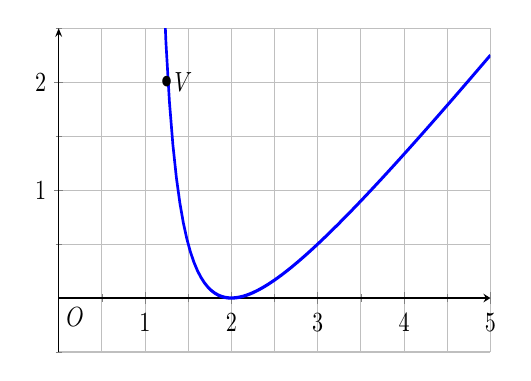
\begin{tikzpicture}[xscale=0.8]
      \begin{axis}%
        [
          grid=both,
          axis equal image,
          minor x tick num=1, % 4 minor ticks => 5 subintervals
          xmin=0,
          xmax=5,
          minor y tick num=1,  % 4 minor ticks => 5 subintervals
          ymin=-.5,
          ymax=2.5,
          axis lines=middle,
          no markers,
          samples=100,
          domain=1:5,
        ]
        \addplot[blue,very thick](x,{(x-2)*(x-2)/(x-1)});
        \draw (axis cs: 0,0)  node[below right]{$O$};
        \draw (axis cs: 1.25,2,25)  node{$\bullet$} node[right]{$V$};
      \end{axis}
    \end{tikzpicture}
  \end{center}
\end{multicols}
  \begin{enumerate}
    \item 
      Pour chacune des abscisses $x$ suivante, calculer $f(x)$, vérifier si $f(x)$ est supérieur à 0,5 ou non, et placer le point d'abscisse $\left( x, f(x) \right)$ sur le graphique, accompagné d'un $V$ si $f(x)\geq0,5$, d'un $F$ sinon.
      \begin{center}
        \begin{tabularx}{\linewidth}{p{2cm}||C|C|C|C|C|C|C}
          $x$ & 1,25 & 1,5 & 2 & 2,5 & 3 & 4 & 5 \\
          \hline
          \hline
          $f(x)$ & 2,25& & & & & & \\
          \hline
          $f(x)\geq0,5$ & Vrai & & & & & \\
        \end{tabularx}
      \end{center}
    \item Observer : Comment peut-on différencier graphiquement les abscisses $x$ telles que $f(x)\geq0,5$ et celles telles que $f(x)\leq0,5$ ?
      \vspace{\stretch{2}}
    \item Quelles sont les solutions de l'équation $f(x)\geq0,5$ ?
      \vspace{\stretch{1}}
    \item Bilan :
      \begin{framed}
        \begin{propriete}Étant donné une fonction $f$, les solutions de l'équation $f(x)\geq k$ (respectivement $f(x)\leq k$) sont \ldots

      \vspace{2cm}
        \end{propriete}
      \end{framed}
  \end{enumerate}
  \end{document}
